\chapter{\ifcpe ทฤษฎีที่เกี่ยวข้อง\else Background Knowledge and Theory\fi}

\section{Model View Controller (MVC)}
โครงงานนี้ใช้ design pattern MVC~\cite{mvc}\CIreply{ทำไมเป็นคำว่า ``และ''}แบ่งออกเป็น 3 ส่วนหลักๆ ดังรูปที่ \ref{mvc} คือ 
\begin{enumerate}
    \item Model
    \item View
    \item Controller
\end{enumerate}


\subsection{Model}
 ในส่วนของ Model จะเป็นการจัดการแปลงจาก Block Code ให้เป็น C\# เพื่อทำให้เกิด Event ต่างๆ เช่นการเดิน, การหมุน
 และการกระโดด เป็นต้น โดยที่ Model จะรับBlock Code มาจาก Controller ในรูปของ JSON
 และจะทำการแปลงเป็น C\# เพื่อสั่งให้ view แสดงผลต่างๆ ส่วนของ Model จะอยู่ใน Unity
 เป็นตัวกลางในการสื่อสารระหว่าง View กับ Controller

\subsection{View}
View นั้นทำหน้าที่แค่แสดงผลโดยรับโค้ดคำสั่งมาจาก Model และทำการแสดงผล จากนั้นจะทำการ
ส่งค่าคืน เพื่อบอก Model ว่าแสดงผลตามตามคำสั่งนั้นแล้ว ในส่วนของ View นั้นจะอยู่ใน
Unity เช่นกัน เพราะ View ใช้แสดงผลกราฟฟิกของ Unity ที่ผู้พัฒนาได้สร้างเอาไว้ เช่น prefabs(รูปแบบสำเร็จ) ต่างๆ ดังรูปที่ \ref{prefabs}
รวมไปถึงการแสดงหน้า UI ของเกม ซึ่งจะกล่าวถึงในหัวข้อ User Interface\par
    

\subsection{Controller}
Controller จะอยู่ทั้ง 2 ฝั่ง คือทั้ง Unity และ WebView โดย Controller ฝั่งหน้าเว็ปจะเป็นการรอให้ผู้ใช้
ลากวางตัว Block Code และเมื่อผู้ใช้กดรัน Controller ฝั่งหน้าเว็ปจะทำการแปลง Block Code ให้เป็น Object 
ในรูปของ JSON และจะถูกนำส่งไปให้ Controller ฝั่ง Unity หลักจากนั้น Controller ฝั่ง Unity จะทำการ
ประมวลผลและแปลงเป็น Object ที่ Unity สามารถอ่านได้เพื่อส่งต่อไปให้ Model


\section{ระบบเกม}
ระบบเกม คือสิ่งที่เป็นระบบที่ให้เกมนั้นทำงานเป็นระบบตามที่เราได้ให้คำสั่งกับตัวโปรแกรมโดยการใช้ภาษาของคอมพิวเตอร์ต่างๆ 
โดยในที่นี้ กลุ่มโครงงานของพวกเราได้ใช้ภาษา C\#\cite{cs} และ JavaScript\cite{js}
ในการเขียนระบบเกมขึ้นมา โดยแบ่งเป็น 2 ส่วน ส่วนแรกคือ C\# ใน Unity 
และ ส่วนที่สองคือ JavaScript ใน WebView(ซึ่งจะกล่าวในหมวดเครื่องมือที่ใช้ในการทำ Blockly ใน Unity) โดยใช้ Localhost ในการ Host\par

\subsection{C\#}
C\# คือ ภาษาคอมพิวเตอร์ประเภท  object-oriented programming พัฒนาโดย
  Microsoft โดยมีจุดมุ่งหมายในการวมความสามารถการคำนวณของ 
C++ ด้วยการโปรแกรมง่ายกว่าของ Visual Basic โดย C\# มีพื้นฐานจาก 
C++ และเก็บส่วนการทำงานคล้ายกับ Java 
C\# ได้รับการออกแบบให้ทำงานกับ .NET platform ของ Microsoft
จุดมุ่งหมายคือ อำนวยความสะดวกในการแลกเปลี่ยนสารสนเทศและบริการผ่านเว็บ 
และทำให้ผู้พัฒนาสร้างโปรแกรมประยุกต์ในขนาดกะทัดรัด C\# 
ทำให้โปรแกรมง่ายขึ้นผ่านการใช้ Extensible Markup Language (XML) 
และ Simple Object Access Protocol (SOAP) 
ซึ่งยอมให้เข้าถึงอ๊อบเจคของโปรแกรมหรือเมธอด 
โดยปราศจากความต้องการให้ผู้เขียนโปรแกรมเขียนคำสั่งเพิ่มในแต่ละขั้นตอน 
เนื่องจากผู้เขียนโปรแกรมสามารถสร้างบนคำสั่งที่มีอยู่ 
แทนที่การคัดลอกซ้ำ C\#
ภาษา C\# ถูกพัฒนาขึ้นโดยเป็นส่วนหนึ่งในการพัฒนาโครงสร้างพื้นฐานของ
.NET Framework เป็นการการนำข้อดีของภาษาต่างๆ 
(เช่นภาษา Delphi , ภาษา C++) มาปรับปรุงเพื่อให้มีความเป็น OOP 
(โปรแกรมเชิงวัตถุ) มากขึ้น ขณะเดียวกันก็ลดความซับซ้อนในโครงสร้างของภาษาลง (เรียบง่ายกว่าภาษา C++) 
และมีสิ่งที่เกินความจำเป็นน้อยลง (เมื่อเทียบกับ Java)~\cite{cs}\par
โดยการที่เราศึกษาและเลือกใช้ ภาษา C\# เพราะว่ามีความเข้ากับตัวโปรแกรม 
Unity 3D ที่เราจะนำมาใช้ในการสร้างออกแบบ ตัวละคร และด่านต่างๆ ภายในเกม\newline
\subsection{JavaScript}
JavaScript คือ ภาษาคอมพิวเตอร์สำหรับการเขียนโปรแกรมบนระบบอินเทอร์เน็ต 
เป็นภาษาสคริปต์เชิงวัตถุ ใช้ในการสร้างและพัฒนาเว็บไซต์ (ใช่ร่วมกับ HTML) 
ซึ่งมีวิธีการทำงานในลักษณะ object-oriented programming มีเป้าหมายในการ 
ออกแบบและพัฒนาโปรแกรมในระบบอินเทอร์เน็ต สำหรับผู้เขียนด้วยภาษา HTML 
สามารถทำงานข้ามแพลตฟอร์มได้ โดยทำงานร่วมกับ ภาษา HTML และภาษา Java 
ได้ทั้งทางฝั่งไคลเอนต์ (Client) และ ทางฝั่งเซิร์ฟเวอร์ (Server)\par
JavaScript ถูกพัฒนาขึ้นโดย เน็ตสเคปคอมมิวนิเคชันส์ 
(Netscape Communications Corporation) 
โดยใช้ชื่อว่า Live Script ออกมาพร้อมกับ Netscape Navigator2.0 
เพื่อใช้สร้างเว็บเพจโดยติดต่อกับเซิร์ฟเวอร์
ต่อมาเน็ตสเคปจึงได้ร่วมมือกับ บริษัทซันไมโครซิสเต็มส์ปรับปรุงระบบ
ของบราวเซอร์เพื่อให้สามารถติดต่อใช้งานกับภาษา Java ได้~\cite{js}\par
พวกเราจึงศึกษาและเลือกใช้ภาษา JavaScript เพราะ 
สามารถทำงานข้ามแพลตฟอร์มได้ โดยสามารถเข้าได้ทั้งกับ Unity และ WebView

\section{โปรแกรมที่ใช้ในการสร้างการออกแบบตัวเกม}
ตัวเกมในของโครงงานของพวกเรา ได้ใช้โปรแกรม Unity3d
ในการออกแบบ UX/UI ของตัวเกมขึ้นมาและทำกราฟฟิกในเกม 
ผ่านการใช้ Asset ของ Unity และ การเขียน Script 
โดยใช้ภาษา C\# ในการพัฒนา\newline
Unity คือ Game Engine ที่ช่วยสร้างเกม 3 มิติ 
และปัจจุบันก็สามารถเกม 2 มิติได้แล้วด้วยซึ่ง 
สามารถทำงานได้ บน 2 แพลตฟอร์ม คือ Windows และ OSX 
และสามารถ Export งานเพื่อนำไปใช้งานได้หลาย แพลตฟอร์ม 
เช่น Windows, OSX, Androids, iOS (iPhone) และ Web\newline
Unity เป็นเครื่องมือช่วยสร้างเกมสามมิติและสองมิติ 
(ข้อ แตกต่างระหว่างโลกสองมิติและสามมิติ คือแกน Z หรือความลึกที่เพิ่มเข้ามา 
พูดง่ายๆก็คือ นอกจากเราจะเคลื่อนที่ ขึ้น/ลง บนหน้าจอได้ ยังสามารถเคลื่อนที่ 
เข้าไปในจอได้)~\cite{unth}
\begin{itemize}
  \item Unity มองทุกอย่างเป็น Game Object ไม่ว่าจะเป็นก้อนหินก้อนหนึ่ง 
  หรือ แมลงตัวหนึ่ง ถือเป็น Game Object โดย Game Object 
  จะทำงานร่วมกับ Component Game Object ที่ปราศจาก Component 
  ก็เหมือนฝุ่นผง ขยับ ไม่ได้ มองไม่เห็นด้วยตาเปล่า ซึ่ง Component 
  เข้ามาเพิ่ม คุณสมบัติและพฤติกรรมให้กับ Game Object ให้สามารถเคลื่อนที่ได้ 
  เปล่งเสียงได้ เป็นต้น
  \item Game Object คือวัตถุต่างๆที่อยู่ในเกม 
  เช่น รถ 1 คัน, สัตว์ 1 ตัว, คน 1 คน, บ้าน 1 หลัง หรือ ต้นไม้ 1 ต้น เป็นต้น 
  นอกจาก Game Object ที่ผ่านตามาบ่อยๆ ในบทความที่ผ่านมาแล้ว 
  ก็ยังมีองค์ประกอบอื่นๆอีก
  \item Component คือคุณลักษณะหรือความสามารถต่างๆ ของ Object เช่น การเคลื่อนไหว
  \item Asset คือ คุณลักษณะภายนอกที่เสริมการทำงานของ Component
  \item Scene คือ ฉากแต่ละฉากซึ่งประกอบด้วย Game Object หลายๆ ตัวรวมกัน
\end{itemize}

\section{เครื่องมือที่ใช้ในการทำ Blockly ใน Unity / เกมคอนโทลเรอร์}
ตัวควบคุมเกมหลักของโครงงานของพวกเรา ได้ใช้ Blockly 
จาก Google for Education ในการทำส่วนของตัวเกมหลักที่ต้องมีการต่อชิ้นส่วน 
Block โดยแต่ละ Block ที่นำมาต่อกันนั้นพวกเราจะสร้างและพัฒนาขึ้นเอง ด้วยภาษา 
JavaScript ผ่าน WebView เพื่อนำไปใช้ในการแสดงผลบน Unity
\GBreply{อธิบายให้มากขึ้น น้อยไป}
\subsection{WebView}
เป็น Asset ที่สามารถให้ผู้ใช้สามารถนำหน้าเว็ปเข้าไปแสดงผลในตัวเกม Unity ได้~\cite{unw}
\subsection{Blockly}
Blockly เป็นผลิตภัณฑ์ของบริษัทกูเกิล ซึ่งมีโปรเจคของบริษัทหรือองค์กรไม่แสวงหากำไร 
ต่าง ๆ นำไปพัฒนาต่อให้เข้ากับผลิตภัณฑ์ของตนเอง เช่น Scratch ที่ใช้ในการเรียนการสอน
ของวิชาวิทยาการคำนวณ
และพวกเราเองก็นำมาใช้เช่นกัน Blockly 
เป็นเครื่องมือที่ช่วยให้การเขียนโปรแกรมนั้นง่ายขึ้น 
เพียงแค่ทำการลากแล้ววางเท่านั้น   Blockly เป็น Library ที่สามารถ
เพิ่มตัวแก้ไขลงลงในแอปพลิเคชันของผู้ใช้ผ่านหลักการคิดการเขียนโปรแกรม
เป็นบล็อคที่เชื่อมต่ออยู่ โดยแสดงผลโค้ดที่ถูกต้องตามหลักไวยากรณ์ในภาษาที่ผู้ใช้เลือก 
ช่วยให้ผู้ใช้สามารถใช้หลักการเขียนโปรแกรมโดยไม่ต้องกังวลเกี่ยวกับไวยากรณ์ 
สามารถใช้งานได้บนในเว็บไซต์ผ่านเครื่องคอมพิวเตอร์ หรือแอปพลิเคชันบน 
ระบบปฏิบัติการ Android หรือ ระบบปฏิบัติการ iOS~\cite{blc}

\GBreply{ไม่ได้ทำ Hosting แล้วลบด้วย}

\section{ความรู้ตามหลักสูตรซึ่งถูกนำมาใช้หรือบูรณาการในโครงงาน}
\begin{itemize}
  \item รู้จัก Block Code จากการเรียนรู้ในวิชา Basic Computer Engineering รหัสวิชา 261103 ซึ่งได้นำ Block Code มาใช้และเป็นแรงบันดาลใจในการทำโครงงานนี้ขึ้นมา
  \item ภาษา HTML และ JavaScript ได้รู้จักและเข้าใจพอสมควร จากการเรียนรู้ในวิชา Basic Computer Engineering Lab รหัสวิชา 261207 นำมาใช้กับการเขียนตัว Controller ที่ใช้ควบคุม Block Code ผ่านการ Hosting ด้วย Localhost
  \item นำหลักการจากวิชา Object-Oriented Programming รหัสวิชา 261200 มาใช้ในการพัฒนาตัวเกมผ่าน Unity
\end{itemize}

\section{ความรู้นอกหลักสูตรซึ่งถูกนำมาใช้หรือบูรณาการในโครงงาน}
\begin{itemize}
  \item Unity3d พวกเราเห็นว่าน่าสนใจและเหมาะสมในการทำเกมเพราะสามารถสร้างเกมที่เป็น 3D จึงได้มีการศึกษาและค้นคว้าข้อมูลเพิ่มเติม รวมถึงฟังก์ชันและการใช้งานโดยรวมทั้งหมด
\end{itemize}

\begin{figure}[h!]
\begin{center}
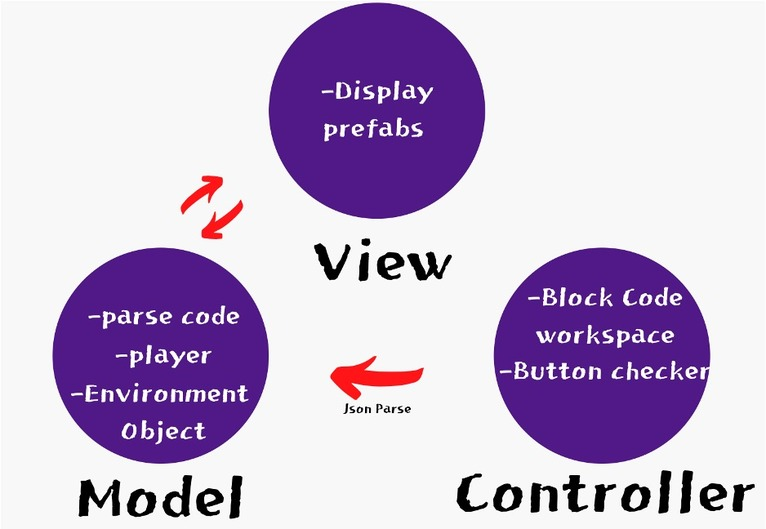
\includegraphics{pic/pic1.jpg}
\end{center}
\caption[Design Pattern MVC]{Design Pattern MVC}
\label{mvc}
\end{figure}

\GBreply{คืออะไร? ทำไมต้องใส่? มองดูละไม่รู้ว่าคือ prefab หรือเอาใส่ใน บท2 หรืออาจจะต้องอธิบายก่อนไหมว่าคืออะไร?}
\begin{figure}[h!]
\begin{center}
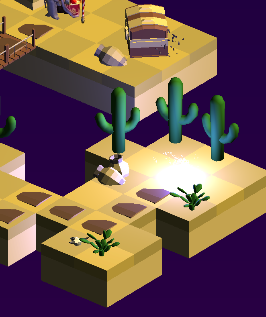
\includegraphics{pic/prefap.PNG}
\end{center}
\caption[ตัวอย่าง prefabs ที่ใช้]{ตัวอย่าง prefabs ที่ใช้ }
\label{prefabs}
\end{figure}
% \subsection{Subsection heading goes here}

% Subsection 1 text

% \subsubsection{Subsubsection 1 heading goes here}
% Subsubsection 1 text

% \subsubsection{Subsubsection 2 heading goes here}
% Subsubsection 2 text

% \section{เครื่องมือที่ใช้ในการทำ Blockly ใน Unity / เกมคอนโทลเรอร์}
% Section 3 text. The dielectric constant\index{dielectric constant}
% at the air-metal interface determines
% the resonance shift\index{resonance shift} as absorption or capture occurs
% is shown in Equation~\eqref{eq:dielectric}:

% \begin{equation}\label{eq:dielectric}
% k_1=\frac{\omega}{c({1/\varepsilon_m + 1/\varepsilon_i})^{1/2}}=k_2=\frac{\omega
% \sin(\theta)\varepsilon_\mathit{air}^{1/2}}{c}
% \end{equation}

% \noindent
% where $\omega$ is the frequency of the plasmon, $c$ is the speed of
% light, $\varepsilon_m$ is the dielectric constant of the metal,
% $\varepsilon_i$ is the dielectric constant of neighboring insulator,
% and $\varepsilon_\mathit{air}$ is the dielectric constant of air.

% \section{About using figures in your report}

% % define a command that produces some filler text, the lorem ipsum.
% \newcommand{\loremipsum}{
%   \textit{Lorem ipsum dolor sit amet, consectetur adipisicing elit, sed do
%   eiusmod tempor incididunt ut labore et dolore magna aliqua. Ut enim ad
%   minim veniam, quis nostrud exercitation ullamco laboris nisi ut
%   aliquip ex ea commodo consequat. Duis aute irure dolor in
%   reprehenderit in voluptate velit esse cillum dolore eu fugiat nulla
%   pariatur. Excepteur sint occaecat cupidatat non proident, sunt in
%   culpa qui officia deserunt mollit anim id est laborum.}\par}

% \begin{figure}
%   \centering

%   \fbox{
%      \parbox{.6\textwidth}{\loremipsum}
%   }

%   % To include an image in the figure, say myimage.pdf, you could use
%   % the following code. Look up the documentation for the package
%   % graphicx for more information.
%   % \includegraphics[width=\textwidth]{myimage}

%   \caption[Sample figure]{This figure is a sample containing \gls{lorem ipsum},
%   showing you how you can include figures and glossary in your report.
%   You can specify a shorter caption that will appear in the List of Figures.}
%   \label{fig:sample-figure}
% \end{figure}

% Using \verb.\label. and \verb.\ref. commands allows us to refer to
% figures easily. If we can refer to Figures
% \ref{fig:walrus} and \ref{fig:sample-figure} by name in the {\LaTeX}
% source code, then we will not need to update the code that refers to it
% even if the placement or ordering of the figures changes.

% \loremipsum\loremipsum

% % This code demonstrates how to get a landscape table or figure. It
% % uses the package lscape to turn everything but the page number into
% % landscape orientation. Everything should be included within an
% % \afterpage{ .... } to avoid causing a page break too early.
% \afterpage{
%   \begin{landscape}
%   \begin{table}
%     \caption{Sample landscape table}
%     \label{tab:sample-table}

%     \centering

%     \begin{tabular}{c||c|c}
%         Year & A & B \\
%         \hline\hline
%         1989 & 12 & 23 \\
%         1990 & 4 & 9 \\
%         1991 & 3 & 6 \\
%     \end{tabular}
%   \end{table}
%   \end{landscape}
% }

% \loremipsum\loremipsum\loremipsum

% \section{Overfull hbox}

% When the \verb.semifinal. option is passed to the \verb.cpecmu. document class,
% any line that is longer than the line width, i.e., an overfull hbox, will be
% highlighted with a black solid rule:
% \begin{center}
% \begin{minipage}{2em}
% juxtaposition
% \end{minipage}
% \end{center}

% \section{\ifcpe%
% ความรู้ตามหลักสูตรซึ่งถูกนำมาใช้หรือบูรณาการในโครงงาน
% \else%
% ISNE knowledge used, applied, or integrated in this project
% \fi
% }

% อธิบายถึงความรู้ และแนวทางการนำความรู้ต่างๆ ที่ได้เรียนตามหลักสูตร ซึ่งถูกนำมาใช้ในโครงงาน

% \section{\ifcpe%
% ความรู้นอกหลักสูตรซึ่งถูกนำมาใช้หรือบูรณาการในโครงงาน
% \else%
% Extracurricular knowledge used, applied, or integrated in this project
% \fi
% }

% อธิบายถึงความรู้ต่างๆ ที่เรียนรู้ด้วยตนเอง และแนวทางการนำความรู้เหล่านั้นมาใช้ในโครงงาน
